\chapter{Concept \& Design}
\label{cha:cod}

This thesis presents the implementation of a practical real world data marketplace for verifiable statistical computations on private datasets. It addresses \emph{Privacy}, \emph{Fairness} and \emph{Regulation} problems of blockchain-based data trading platforms, while the focus is on \emph{Privacy}. \emph{Furthermore, I only focus on static tabular datasets with very infrequent changes. Hence, I do \textbf{not} focus on real-time streaming data and training of machine-learning models}. My proposed implementation implicitly targets the \emph{Data Transfer} and \emph{Payment} process as well as \emph{IAM} -- some of the fundamental functional requirements, as already depicted in Figure \ref{fig:components}. Specifically, I construct a secure blockchain-based data trading ecosystem, using Blockchain as a medium to (i.) prevent single-point of failure; (ii.) define data usage policies; (iii.) create a transparent, non-repudiable and tamper-proof log of transactions; and (iv.) enforce a fair data exchange protocol. However, the \emph{focus} of this thesis is rather on creating a generic mechanism to make a variety of computations on arbitrary private datasets verifiable, and Blockchain is a necessary part of the puzzle. This thesis uses Verifiable Off-chain Computation (VOC) to address this problem \cite{eberhardtOffchainingModelsApproaches2018,eberhardtBlockchainInsightsOffChaining2017}.

VOC is a derivative of Verifiable Computation and aims to secure the integrity of computations performed by untrusted parties off the Blockchain. The result of the computation is then published to the Blockchain and verified on-chain with a cryptographic proof, attesting its correctness. Off-loading the computation has multiple benefits -- (i.) it increases the scalability by avoiding complex redundant computations on each node; (ii.) it reduces on-chain transaction costs by significantly lowering the size of transactions; and (iii.) it improves privacy by hiding PII and confidential data from the public ledger. \cite{eberhardtOffchainingModelsApproaches2018,eberhardtZoKratesScalablePrivacyPreserving2018a,simunicVerifiableComputingApplications2021,xuSlimChainScalingBlockchain} 

According to \cite{eberhardtOffchainingModelsApproaches2018}, a reasonable VC scheme for off-chain computations needs to fulfill the following requirements: (i.) non-interactivity; (ii.) cheap verification; (iii.) weak security assumptions; and (iv.) zero-knowledge. ZkSNARKs, ZkSTARKs and Bulletproofs provide a valid approach to the aforementioned requirements. ZkSNARKs are a type of Zero-knowledge proof (ZKP) that are \emph{non-interactive} and \emph{succinct}. \emph{Non-interactivity} defines the possibility to convince a verifier of a particular statement with only \emph{one} message \cite{eberhardtOffchainingModelsApproaches2018,eberhardtZoKratesScalablePrivacyPreserving2018a,simunicVerifiableComputingApplications2021}. \emph{Succinct} defines a proof that is small in size, compared to ZkSTARKs and Bulletproofs, and can be verified cheaply and quickly, typically within a few milliseconds \cite{simunicVerifiableComputingApplications2021}. This thesis uses a ZKP with ZkSNARKs for verifiable computations on private datasets.

The proposed blockchain-based data trading platform is designed for two party relationships between a buyer \emph{B} and seller \emph{S}. The current high-level protocol for a trade between \emph{B} and \emph{S} on the proposed platform is described by the following exemplary use case and shown in the subsequent Figure \ref{fig:usecase}, without technical details.

\begin{figure}[!htb]
    \centering
    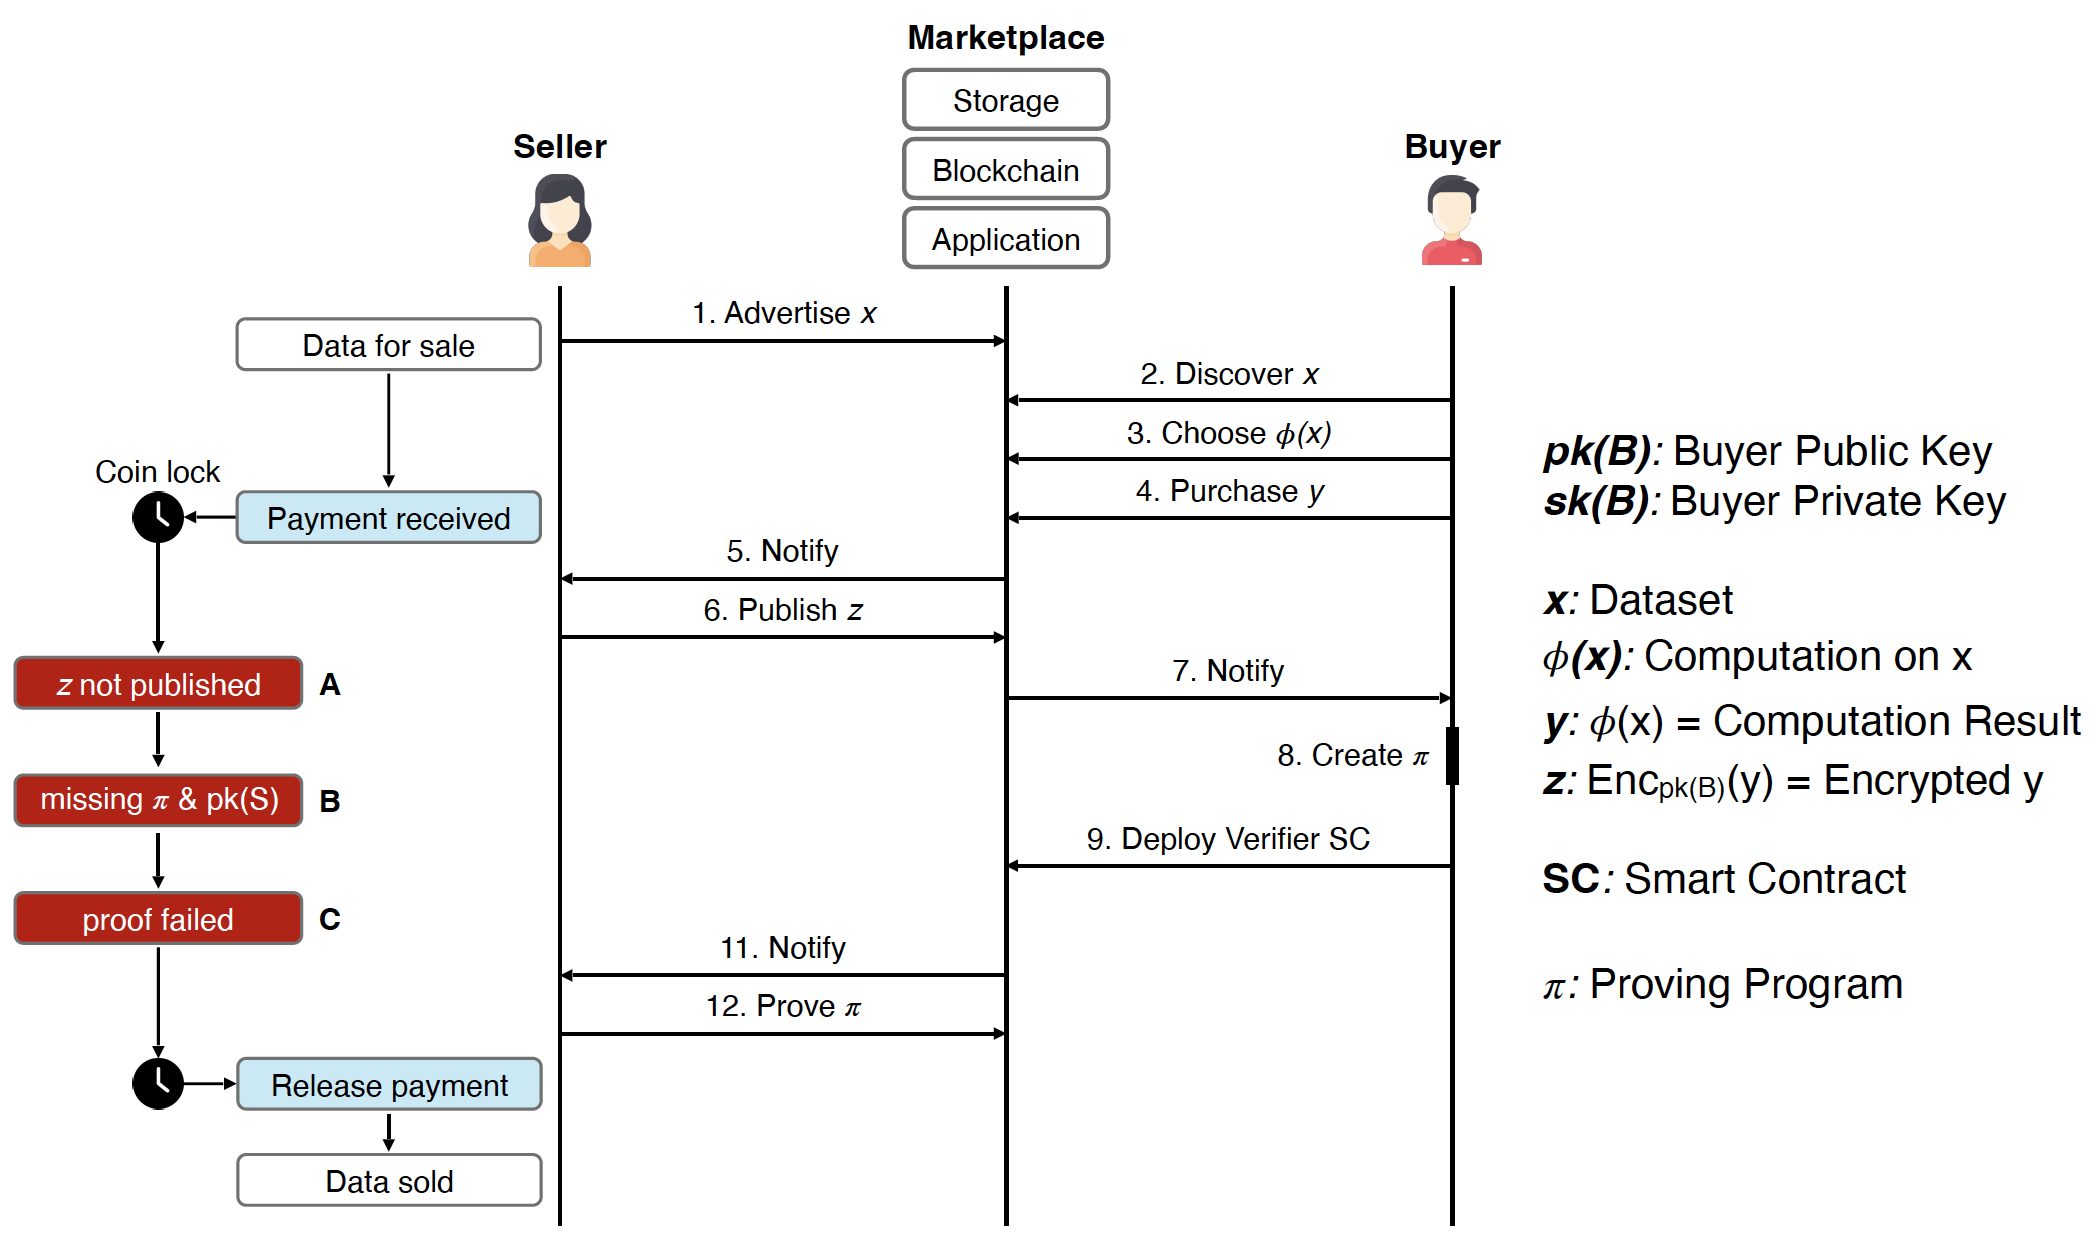
\includegraphics[width=14cm]{images/protocol.png}
    \caption{Proposed protocol for a blockchain-based data trading platform with Compute-to-Data and Verifiable Off-chain Computation for verifiable statistical queries on private datasets. The marketplace between a buyer \emph{B} and seller \emph{S} is highly abstracted into storage, Blockchain and application components, which are necessary for the entire data marketplace ecosystem.}
    \label{fig:usecase}
\end{figure}

\subsubsection{Example}

S advertises a dataset $x$ about health information of a population on the marketplace. The dataset $x$ is described by metadata, i.e. the time interval, data category, amount of columns and rows as well as the header of each column, among other metadata. The actual content of the dataset is hidden from the buyer. A potential \emph{B} enters the data marketplace and is interested in receiving the average age of cancer diagnosed patients in 2021. He or she discovers a promising dataset $x$ of \emph{S} in the health category, containing all cancer diagnosed patients worldwide. \emph{B} chooses to purchase the desired computation $\phi(x)$ for the \emph{age} column. He or she commits the purchase by an on-chain transaction, including the given price by \emph{S}. All coins are now temporarily locked in a smart contract. \emph{S} subsequently gets notified by the purchase and calculates the average on a private node of \emph{S}, protecting privacy and confidentiality of \emph{S}'s dataset. \emph{S} transfers the result $z = Enc_{pb(B)}(y=\phi(x))$ to the Blockchain, encrypted with the public key of \emph{B}. \emph{B} gets notified and decrypts the result with his or her private key $Dec_{sk(B)}(z)$. \emph{B} is now uncertain about the correctness of the result and therefore constructs a program $\pi$ for the seller to prove (i.) the correctness of the computation; (ii.) the result originates from the advertised dataset; and (iii.) the proof is given by the seller. He or she then publishes a smart contract for the verification of the proof. \emph{S} is now responsible to generate such a proof for the verifier smart contract, to transparently proof all the requirements of $\pi$. According to that, the execution of the protocol terminates in the following situations:

\newpage
\begin{enumerate}
    \item \emph{S} finally manages to submit a valid proof to the verifier contract. In this case, the payment is released to \emph{S}.
    \item \emph{S} does not publish a computation result. In this case, \emph{B} can withdraw his payment after a timeout. \textbf{(Scenario A)}
    \item \emph{B} does not construct a proving program and does not publish the proving key to \emph{S}. In this case, \emph{S} can withdraw the payment after a timeout. \textbf{(Scenario B)}
    \item \emph{S} is not able to submit a valid proof to the verifier contract. In this case, \emph{B} can withdraw his payment after a timeout. \textbf{(Scenario C)}
\end{enumerate}

\noindent \textbf{Note}: This protocol is only a first idea and the final protocol may highly differ. At the time of writing this exposé I already noticed that there is one major weakness in the current protocol. A malicious \emph{B} could send a fake proving key to \emph{S}, so that it is impossible for \emph{S} to construct a valid proof. According to that, \emph{B} would always be able to withdraw his payment, if he has no honest interest in actually verifying the correctness of his purchased values. While this is not the focus of this thesis, I will try to create a completely trustless protocol between \emph{B} and \emph{S}.